\section{问题三：全向七点覆盖与环半径收缩}
\label{new:sec-q3}
\subsection{从900米覆盖基线到可调七点构型}
记源区域为$\disk=\{g:\norm g\le R\}$，其中$R=1800$米，接收半径的题给下界为1000米。全向发现只需保证每个可能源位置至少落入一个检测点的接收圆盘；但覆盖半径越小，并不意味着式\eqref{eq:time}中的总时间越少。为分离覆盖安全性与行程代价，考虑原点加正六边形环的同一构型族：
\begin{equation}\label{new:eq-seven-points}
p_0=(0,0),\qquad p_{k+1}=d\,u(k\pi/3),\quad k=0,\ldots,5,
\qquad u(\theta)=(\cos\theta,\sin\theta).
\end{equation}
原始保守基线取$d=900\sqrt3$，最终策略取$d=1200$。两者均保留七个检测位置，变化的是完整覆盖所需的圆盘半径，而不是逐频道排查的逻辑。

\begin{theorem}[七点构型的精确覆盖半径]\label{new:thm-ring-cover}
对$1200\le d\le900\sqrt3$，式\eqref{new:eq-seven-points}在$\disk$上的精确覆盖半径为
\begin{equation}\label{new:eq-ring-radius}
\rho(d)=\max_{g\in\disk}\min_{0\le j\le6}\norm{g-p_j}
=\max\left\{\frac d{\sqrt3},\sqrt{R^2+d^2-\sqrt3Rd}\right\}.
\end{equation}
特别地，$\rho(900\sqrt3)=900$，故原900米圆盘覆盖基线成立。
\end{theorem}
\begin{proof}
将源写为$g=r\,u(\theta)$。总有一个环点与之极角相差不超过$\pi/6$；固定$r$时，相邻环点的角平分线给出到最近环点的最坏距离。因此该圆周上到最近检测点的最大距离恰为
\begin{equation}\label{new:eq-ring-envelope}
f_d(r)=\min\left\{r,\sqrt{r^2+d^2-\sqrt3dr}\right\}.
\end{equation}
两项在$r=d/\sqrt3$相等，此前原点更近，此后环点更近。在$[d/\sqrt3,R]$上，后一项的平方是凸二次函数，其最大值位于两个端点；在$[0,d/\sqrt3]$上，$f_d(r)=r$。于是全域最大值为式\eqref{new:eq-ring-radius}。两端值均在角平分线上实际达到，故该式不是仅有充分性的上界，也不依赖空间网格采样。代入$d=900\sqrt3$后两项均为900米，证明包含圆周边界和扇区接缝。
\end{proof}

由式\eqref{new:eq-ring-radius}，给定安全覆盖半径$q\ge R/2$时，需要同时满足
\begin{equation}\label{new:eq-ring-feasible}
d\le\sqrt3q,\qquad
\frac{\sqrt3R-\sqrt{4q^2-R^2}}2\le d\le
\frac{\sqrt3R+\sqrt{4q^2-R^2}}2.
\end{equation}
当$q=900$时，这些条件将环半径固定为$900\sqrt3$；允许覆盖半径向物理下界1000米靠近，则可以向内收缩检测环。最终采用$d=1200$米，解析式给出
\begin{equation}\label{new:eq-ring-margin}
\begin{aligned}
\rho(1200)&=\sqrt{1800^2+1200^2-\sqrt3\cdot1800\cdot1200}
\approx968.901572\ \mathrm m,\\
1000-\rho(1200)&\approx31.098428\ \mathrm m.
\end{aligned}
\end{equation}
因而收缩后仍保留约31.098米距离余量。若理想检测点到实际检测位置的总欧氏偏差不超过$\eta$，三角不等式给出实际覆盖半径至多为$\rho(1200)+\eta$；例如$\eta\le1$米时仍严格小于1000米。这里的余量属于全局发现骨架，与示向度误差和局部清除半径是不同的量。

\subsection{骨架路径代价与七点下界的适用范围}
从原点出发、访问全部六个环点而不要求返回时，纯骨架路径的精确最短长度为
\begin{equation}\label{new:eq-ring-path}
L_{\rm ring}^{\min}(d)=6d.
\end{equation}
起点到首个环点必须走$d$；任意两个不同环点的距离至少为相邻点弦长$d$，故其后五次转移各至少走$d$。沿圆周依次访问即可达到该下界。插入额外中间停靠点不能突破这一界，因为折线路径不短于对应直线。因此，环收缩使完整纯骨架路线由$5400\sqrt3$米变为7200米。在所用参数区间内，$\rho(d)$由边界项控制，且
\[
\rho'(d)=\frac{d-\sqrt3R/2}{\sqrt{R^2+d^2-\sqrt3Rd}}\le0,
\qquad \frac{\mathrm d L_{\rm ring}^{\min}}{\mathrm d d}=6.
\]
这说明扩大环半径能改善最坏覆盖距离，却增加骨架行程；收缩则作相反交换。式\eqref{new:eq-ring-path}不包含定位支线、检测与切换费用，也不适用于达到16源上界后省略余点的路线，故其差额不能直接充当每局实际节省时间。

\begin{theorem}[900米覆盖要求下至少需要七点]\label{new:thm-seven-lower}
用半径900米的闭圆盘覆盖半径1800米的整个圆域，至少需要七个圆盘；式\eqref{new:eq-seven-points}在$d=900\sqrt3$时达到此下界。
\end{theorem}
\begin{proof}
设一个检测圆盘的圆心距原点为$t>0$，与源圆周的交弧角半宽为$\beta$。有交弧时余弦定理给出
\[
\cos\beta=\frac{R^2+t^2-q^2}{2Rt}
=\frac1{2R}\left(t+\frac{R^2-q^2}{t}\right)
\ge\frac{\sqrt{R^2-q^2}}R,
\quad q=900.
\]
所以$\beta\le\arcsin(q/R)=\pi/6$，等号仅在$t=\sqrt{R^2-q^2}=900\sqrt3$时成立。圆心为原点的900米圆盘不与源圆周相交。六个圆盘若覆盖整条圆周，六条交弧都必须达到最大角宽$\pi/3$，且不能有正长度重叠。于是六个圆心均在半径$900\sqrt3$的环上，按$\pi/3$间隔排列；然而它们距原点均大于900米，不能覆盖原点。六个及更少圆盘均不可能覆盖全域，结合前述七点构造即得结论。
\end{proof}
这一精确下界只针对900米覆盖要求。将允许半径改为1000米后，最大交弧变宽，上述等号论证不再成立；因此本文没有证明物理接收半径下任意布局仍至少需要七点，也不把$d=1200$称为连续参数空间的全局最优值。最终采用的七点环是在完整发现保证下减少骨架移动的明确构造，其任务时间表现另由冻结策略的实验评价。

\section{问题四：具有严格方向余量的25点双环覆盖}
\label{new:sec-q4}
\subsection{由近邻覆盖转向方向覆盖}
定向源不仅要求检测点距源不超过接收半径，还要求检测点位于发射前方。设源的单位发射法向为$n$，前方闭半平面为$n^{\mathsf T}(p-g)\ge0$。边界源若朝圆外发射，圆内近邻点可能全部位于背面，因此问题三的距离覆盖不能直接用于问题四。题目允许提交源圆域外的机器人位置，本文利用这一条件重新设计骨架，而不把外部检测点投影回圆内。

历史\texttt{enhanced}对照保留边长990米的31点三角格，配合原有滚动骨架排序、分离式调度和全部未清除频道扫描。该格点集合的逐点不可删性，说明从\emph{固定的31点集合}直接删除一个点可能失去覆盖见证；它并不意味着任意布局都至少需要31点。最终\texttt{refined}采用下面独立证明的25点双环，其改进来自重新布点而不是未经证明的删点。

取$a=940$米、$b=1870$米，定义原点、内环和外环为
\begin{equation}\label{new:eq-polar-points}
\begin{aligned}
p_0&=O=(0,0),\\
p_{1+k}&=I_k=a\,u(k\pi/6),\\
p_{13+k}&=E_k=b\,u(k\pi/6+\pi/12),\qquad k=0,\ldots,11.
\end{aligned}
\end{equation}
内环角间隔为$30^\circ$，外环相对内环错开$15^\circ$。共有13个点在源圆域内，12个点在圆域外。索引只标识覆盖义务，不规定访问顺序。

\subsection{36个闭三角形组成的有限覆盖证书}
令所有下标按模12计算，构造三类闭三角形
\begin{equation}\label{new:eq-triangulation}
\begin{aligned}
T_k^{(1)}&=\conv\{O,I_k,I_{k+1}\},\\
T_k^{(2)}&=\conv\{I_k,E_k,I_{k+1}\},\\
T_k^{(3)}&=\conv\{I_{k+1},E_k,E_{k+1}\}.
\end{aligned}
\end{equation}
这36个三角形完整剖分外正十二边形$H=\conv\{E_0,\ldots,E_{11}\}$。具体而言，第一类剖分内正十二边形；内外连接线分别位于端点极角确定的$15^\circ$扇区，不同扇区内部互不相交。外端点位于相应内边支撑线之外，而$a<b\cos(\pi/12)$保证内点严格位于相应外边内侧。因此后两类恰好填满内外多边形之间的环带，不产生交叉边或孔洞。所有三角形按式中顺序逆时针定向，内部边成对反向出现，余下边界正是外十二边形；25个顶点、60条无向边与36个面还满足$25-60+36=1$。边计数是有限结构的核对，而完整性依赖上述无交叉剖分。

记$c=\cos(\pi/12)$、$s=\sin(\pi/12)$。剖分中只有四种边长：
\begin{equation}\label{new:eq-four-lengths}
\begin{aligned}
\ell_0&=a,& \ell_I&=2as,\\
\ell_E&=2bs,& \ell_{IE}&=\sqrt{a^2+b^2-2ab c}.
\end{aligned}
\end{equation}
任一三角形的直径等于其最长边，故只需给出这四种边长的共同上界。利用精确根式
\[
c=\frac{\sqrt6+\sqrt2}{4},\qquad s=\frac{\sqrt6-\sqrt2}{4},
\]
以及可由平方比较得到的$1.4142<\sqrt2<1.4143$、$2.4494<\sqrt6<2.4495$，可得有理界
\begin{equation}\label{new:eq-trig-bounds}
c>\frac{9659}{10000},\qquad \frac14<s<\frac{259}{1000}.
\end{equation}
以下比较均使用有限有理数，不依赖浮点近似决定不等号方向：
\begin{equation}\label{new:eq-polar-bounds}
\begin{aligned}
bc&>1870\cdot\frac{9659}{10000}=1806.233>1805,\\
\ell_0&=940<993,\qquad \ell_I<486.92<993,\\
\ell_E&<968.66<993,\\
\ell_{IE}^2&<940^2+1870^2-2\cdot940\cdot1870\cdot\frac{9659}{10000}\\
&=984781.96<993^2=986049.
\end{aligned}
\end{equation}
因此每个闭三角形的直径$D_T<993$米，而外十二边形的内切圆半径$bc>1805$米，特别有$B(O,1805)\subset H$。这两个严格界分别控制接收距离与源边界之外的辅助空间。

\begin{theorem}[25点的任意方向鲁棒覆盖]\label{new:thm-direction-cover}
对任意$g\in\disk$、任意单位发射法向$n$，式\eqref{new:eq-polar-points}中至少有一个点$v$，使得其实际检测位置$v'$在满足$\norm{v'-v}\le1$米时仍有
\begin{equation}\label{new:eq-direction-margin}
n^{\mathsf T}(v'-g)\ge4\ \mathrm m,
\qquad \norm{v'-g}<999\ \mathrm m.
\end{equation}
故该点严格位于发射前方，且严格处于题给最小接收半径1000米以内。
\end{theorem}
\begin{proof}
取仅用于证明的辅助点$h=g+5n$。由$\norm h\le1805$及式\eqref{new:eq-polar-bounds}，有$h\in H$，故$h$属于剖分中的某个闭三角形$T$。写成重心组合
\[
h=\sum_{i=1}^3\lambda_i v_i,\qquad
\lambda_i\ge0,\quad\sum_{i=1}^3\lambda_i=1.
\]
投影满足
\begin{equation}\label{new:eq-shift-projection}
\sum_{i=1}^3\lambda_i n^{\mathsf T}(v_i-g)
=n^{\mathsf T}(h-g)=5.
\end{equation}
所以至少一个正权重顶点$v$满足$n^{\mathsf T}(v-g)\ge5$。又因$v,h\in T$，
\[
\norm{v-g}\le\norm{v-h}+\norm{h-g}\le D_T+5<998.
\]
加入不超过1米的总位置偏差后，由柯西不等式与三角不等式得
\[
n^{\mathsf T}(v'-g)\ge5-\norm{v'-v}\ge4,
\qquad
\norm{v'-g}\le\norm{v-g}+\norm{v'-v}<999.
\]
这就证明了式\eqref{new:eq-direction-margin}。
\end{proof}

上述证明不要求源$g$与辅助点$h$位于同一个三角形，也不需要在线知道$g$或$n$。源在圆周上并朝外发射、源在原点或内环点、辅助点恰落在三角形边或顶点等情况均包含在闭三角形论证中。正投影下界还排除了所选点与源重合的退化情形，不需依赖零距离方位定义或恰好落在发射边界上的浮点判断。1米是理想点到实际测量位置的\emph{总欧氏误差预算}，包括坐标计算、传输舍入和实际位置偏差之和；不能对每一种误差分别重复使用1米。仅将两个坐标四舍五入到整米所造成的误差至多$\sqrt{1/2}$米，但仍须计入其余误差。

\begin{figure}[htbp]\centering
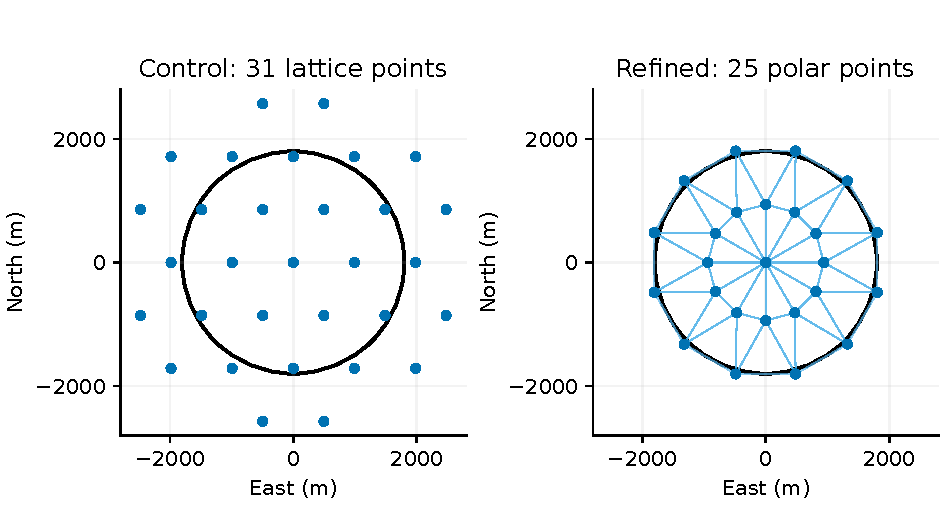
\includegraphics[width=\textwidth]{figures/research_coverage.pdf}
\caption{问题四发现骨架的同尺度比较：左为历史31点三角格，右为最终25点错相双环及36个闭三角形。源区域均为半径1800米圆盘；右图外十二边形包含辅助半径1805米圆盘，圆外点是方向覆盖义务的一部分。}
\label{new:fig-coverage}
\end{figure}

\subsection{可实现路线、有限核验与点数结论}
双环给出一条显式开放扫描路线
\[
O,I_0,I_1,\ldots,I_{11},E_{11},E_{10},\ldots,E_0,
\]
其长度为
\begin{equation}\label{new:eq-polar-route}
L_{25}=a+22(a+b)\sin(\pi/12)+\sqrt{a^2+b^2-2ab\cos(\pi/12)}.
\end{equation}
它恰访问每个点一次，不要求回到原点。保存的独立研究核验给出最大边长约992.316061米、该显式路线长度约17932.509429米，并核对了36个三角形、60条边及无交叉完整剖分。这些数值与实现检查补充解析证书，不替代定理中的全称证明；式\eqref{new:eq-polar-route}也只是一条可行路线，不是旅行商最优值或联合调度的实际路径预测。

在20个频道都需完成全骨架扫描的义务计数下，31点对应$31\times20=620$次检测，25点对应500次，少120次检测，即式\eqref{eq:time}的检测项少600秒。实际任务会提前清除频道并跳过部分已知源补测，还可能增加定位分支；因此600秒不是每局固定节省，路线和切换收益也须独立核算。另一方面，本文没有证明25点是任意非规则布局、任意层数或任意方向覆盖方法中的全局最少点数。可成立的结论是：31点固定格不可删与25点重新设计可覆盖并不矛盾，后者提供了点数更少且留有明确扰动余量的完整发现骨架。

\section{联合调度、扫描筛选与逐频道停止证书}
\label{new:sec-dispatch}
\subsection{在共同任务路线中选择下一项}
分开评价一个待扫描骨架点或一个已知源，会忽略执行当前任务后与其他任务的位置关系。最终策略将二者放入同一个开放路线：令当前位置为$q$，每个未完成骨架任务的代理点为其检测坐标、半径为0；每个已发现未清除频道$c$的代理点为保守区域$P_c$的最小包围圆中心$z_c$，半径为$r_c$。对全部$n$个任务的排列$\pi$定义
\begin{equation}\label{new:eq-route-proxy}
J_\gamma(\pi)=\norm{q-z_{\pi_1}}
+\sum_{j=1}^{n-1}\norm{z_{\pi_{j+1}}-z_{\pi_j}}
+\gamma r_{\pi_1}.
\end{equation}
问题三取$\gamma=0$，对应\texttt{center}；问题四取$\gamma=1$，对应\texttt{guarded}。后者只在首项为目标时增加其半径，抑制立即向一个不确定中心作长距离承诺；半径不是障碍半径，也不是未来真实任务时间的误差界。该代理不含未知的后续示向、光学尝试和频道切换，最终优劣仍以式\eqref{eq:time}评价。

实现先用最近插入法构造完整排列：首项最小化当前位置距离加首项惩罚，此后选离已有路线最近的未插入任务，将其放入代理增量最小的空隙。再进行至多$n$轮2-opt扫描，每轮按固定次序检查连续区间反转，只接受严格改善的首个交换；没有改善即停止。开放路线不增加返回起点的虚拟边，反转从首项开始时还须计入半径惩罚的变化。距离矩阵占$O(n^2)$空间，最近插入耗时$O(n^2)$，每轮2-opt检查$O(n^2)$个区间，总时间上界$O(n^3)$。轮数上限保证计算量可控，但不保证到达局部或全局最优。

每次只执行排列首项，依据已接受动作确定的新位置与新观测重建任务集。选中目标仍调用既有局部定位与完整光学后备，不在代理中心直接假定清除成功。任务按类型和频道或骨架索引区分，即使坐标重合也不合并；插入和反转都保持全部输入任务。因此联合调度改变访问顺序，不会删除无源认证所需的骨架义务。

\subsection{区分首次发现义务与已知源的补测价值}
骨架扫描先剔除已确认成功清除的频道，并优先检测当前测向机频道，再按频道编号排序，以避免一次不必要的初始切换。对其余频道采用以下准确规则：
\begin{itemize}
\item 问题三的\texttt{unknown}规则：尚未建立源轨迹的频道必须检测；已有正测向轨迹的未清除频道跳过骨架补测，保留为独立定位清除任务。
\item 问题四的\texttt{useful}规则：未知频道仍必须检测；对已有轨迹的频道，在骨架点$p$仅当$r_c>19.9$且$\norm{p-z_c}-r_c\le1500$时补测。换言之，$r_c\le19.9$或$\norm{p-z_c}-r_c>1500$才跳过；距离下界恰为1500时不跳过。
\end{itemize}
第二条中，$r_c\le19.9$表示已具备既有局部清除条件；由$P_c\subseteq B(z_c,r_c)$可知，$\norm{p-z_c}-r_c>1500$时整个保守区域都超过最大电磁接收距离，补充示向没有价值。反向条件只表示可能有用，不保证定向源处于发射前方。局部任务完成后的停靠共享同样保留区域大小与1500米筛选，并额外跳过该频道曾在\emph{完全相同坐标}检测过的位置；此去重条件不被误写为\texttt{useful}骨架扫描本身的条件。

两种规则都不跳过未知频道的必需检测。已知源从骨架扫描中省下的观测不算作无信号，也不填入已完成索引集合；其完成义务由“发现”转为“收到该频道成功清除反馈”。尤其在问题四，\texttt{no\_signal}可以来自距离过远或位于发射背面，不能据此删除1000米位置圆盘，也不能将已知源改判为不存在。

\subsection{安全停止不依赖启发式代理是否准确}
记$V$为当前完整骨架索引集，问题三为$\{0,\ldots,6\}$，最终问题四为$\{0,\ldots,24\}$；$V_c$只记录该频道已接受的实际骨架检测。定义频道完成证书
\begin{equation}\label{new:eq-stop-certificate}
\operatorname{Cert}_c=
\begin{cases}
C,&\text{已收到频道$c$的\texttt{success}清除反馈},\\
N,&\text{从未发现该频道源，且全部$V$上的有效检测均无信号},\\
U\text{或}D,&\text{尚未确定或已发现未清除}.
\end{cases}
\end{equation}
若一个从未发现的频道在$V_c=V$后仍全部无信号，则假设其有源将与问题三或问题四的覆盖定理矛盾，故$N$证书可靠；一旦进入$D$状态，只能以成功清除完成，不能转成$N$。合法停止条件为
\begin{equation}\label{new:eq-stop}
\bigl[\forall c\in\{1,\ldots,20\},\ \operatorname{Cert}_c\in\{C,N\}\bigr]
\quad\text{或}\quad
\bigl[\#\{c:\operatorname{Cert}_c=C\}=16\bigr].
\end{equation}
第二项利用题给总数上界，统计的是16个不同频道的成功清除；已清除10个、队列暂时为空或长时间没有新发现均不满足停止条件。动作异常或时间中断也不能替代证书。

式\eqref{eq:poly}的真实源包含关系仅依赖先验和实际返回的有效正观测，不依赖选点代理是否准确。联合调度不改写观测，扫描筛选不虚构负证据，定向失信号不作不安全的位置删减；因此这些效率层动作不会破坏既有几何包含不变量。配合保留的有限局部测向和完整光学覆盖，发现、清除与停止分别拥有可核查的依据，而效率由真实执行的$L,M,S,F,K$统一结算。
